\subsection{Overview}
In the following section, mockups for the graphical user interface (GUI) are presented.  
Some basic mockups can be seen in RASD document, with a few basic screen concepts being presented for both Android and iOS app versions. \newline

In this document mostly one version of the app will be shown since they are nearly identical, with the only differences being due to native button placements on respective operating systems, which are not related to the app. \newline
 
The base design and colours are taken from RASD. Several new menu screens have been added and some old ones have been modified.  

The main aim of the design was simplicity and ease of use. Since we want to make this app available to as many customers as possible, it is important that even people who do not have a lot of experience with different apps have no trouble using it. \newline 

Every button has been made bigger and the size of letters is larger than usually in other apps. There is no excess information at the screen at any time and the navigation is rather simple and logical.  \newline

Minimal amount of design elements has been used in order to make the app look a little bit more stylish without sacrificing efficiency. Besides the base ones, colours have solely been used to showcase validity of a certain action.  \newline


There is also a possibility of adding colorblind mode and a help screen, which will show and explain basic functions of the application and how to use them. This would be highly recommended when implementing the app. \newline

In the text we will mostly be referring to the iPhone devices, although the app is supposed to work on all iOS supported devices. This is due to the fact that people will most likely use this app on iPhone devices and not on iPad and iPod devices. Terms iOS and iPhone could for that reason be used interchangeably in the further text.
\newpage
\subsection{Proposed design}

\captionsetup{justification=centering}
\begin{itemize}
\item Already proposed icon look for the app on both Android and iOS devices featured in RASD.
\begin{figure}[!htb]
\centering
\begin{minipage}{0.4\textwidth}
\centering
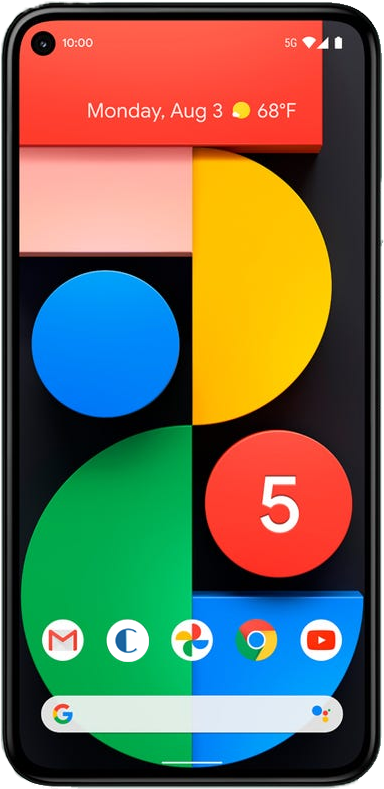
\includegraphics[width=0.65\textwidth]{Images/App/Android_AppIcon}
\caption{\label{fig:androidappicon}\textbf{Android icon concept}}
\end{minipage}
\begin{minipage}{0.4\textwidth}
\centering
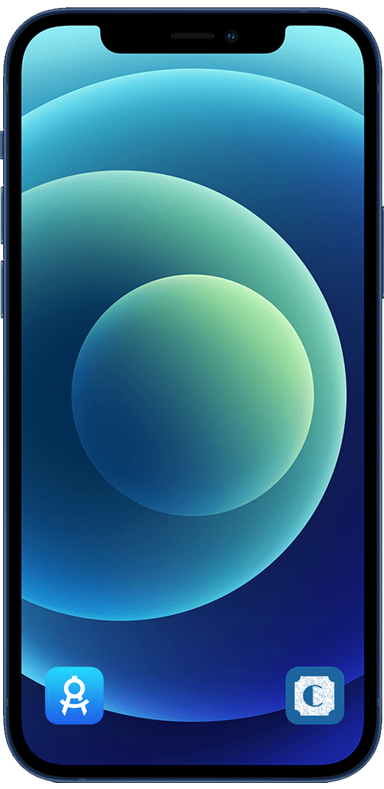
\includegraphics[width=0.65\textwidth]{Images/App/iPhone_AppIcon}
\captionsetup{justification=centering}
\caption{\label{fig:iphoneappicon}\textbf{iPhone icon concept}}
\end{minipage}
\end{figure}

\item Already proposed title screen concepts featured in RASD. First step when entering the app is selecting the desired store.
\begin{figure}[!htb]
\centering
\begin{minipage}{0.4\textwidth}
\centering
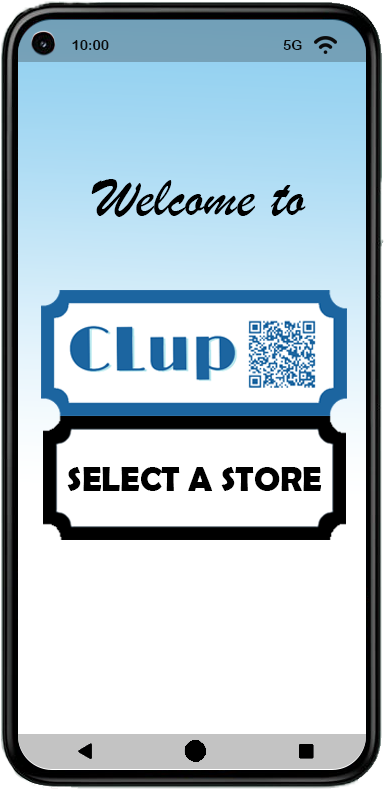
\includegraphics[width=0.65\textwidth]{Images/App/Android_HomeScreenv2}
\caption{\label{fig:androidhomescreen}\textbf{Android home screen}}
\end{minipage}
\begin{minipage}{0.4\textwidth}
\centering
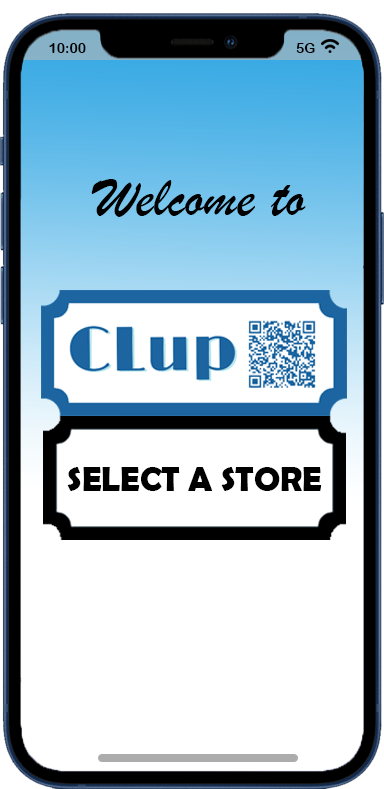
\includegraphics[width=0.65\textwidth]{Images/App/iPhone_HomeScreenv2}
\captionsetup{justification=centering}
\caption{\label{fig:iphonehomescreen}\textbf{iPhone home screen}}
\end{minipage}
\end{figure}
\end{itemize}

Following proposed concepts are shown only on Android devices, however, just as already mentioned, they are practically identical to the iPhone version.

\begin{itemize}
\item Main screen selection of the app, featuring selection for all most vital functions of the app. 
\begin{figure}[!htb]
\centering
\begin{minipage}{0.4\textwidth}
\centering
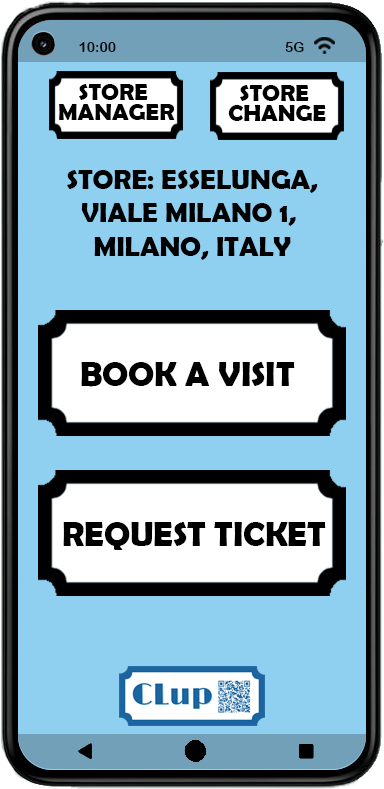
\includegraphics[width=0.65\textwidth]{Images/App/Android_MainScreenv3}
\caption{\label{fig:androidmainscreen}\textbf{App main screen}}
\end{minipage}
\begin{minipage}{0.4\textwidth}
\centering
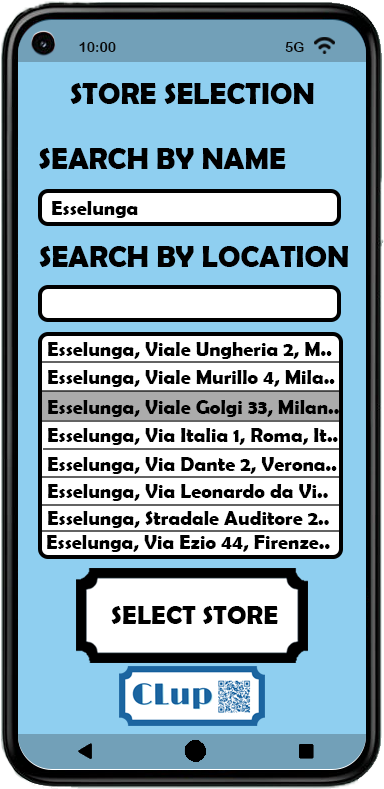
\includegraphics[width=0.65\textwidth]{Images/App/Android_StoreSelection}
\captionsetup{justification=centering}
\caption{\label{fig:androidstoreselection}\textbf{App store selection}}
\end{minipage}

\end{figure}
\item Login screen for the store manager and generated ticket screen.
\begin{figure}[!htb]
\centering
\begin{minipage}{0.4\textwidth}
\centering
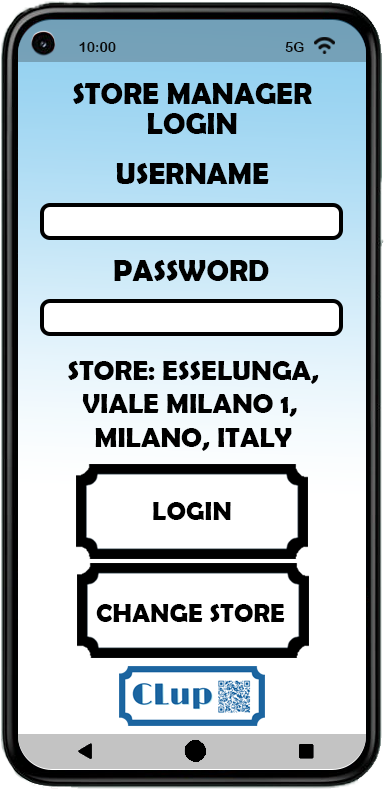
\includegraphics[width=0.65\textwidth]{Images/App/Android_LoginManager}
\caption{\label{fig:androidlogin}\textbf{App store manager login screen}}
\end{minipage}
\begin{minipage}{0.4\textwidth}
\centering
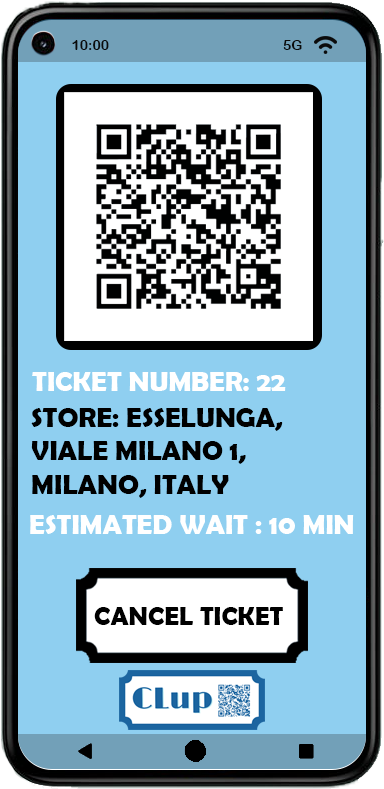
\includegraphics[width=0.65\textwidth]{Images/App/Android_RequestTicket}
\captionsetup{justification=centering}
\caption{\label{fig:androidticket}\textbf{App ticket request screen}}
\end{minipage}
\end{figure}
\end{itemize}
\newpage

\begin{itemize}
\item "Book a visit" feature has an implemented calendar for date selection and a list of available timeslots for a selected date in a certain store.
\begin{figure}[!htb]
\centering
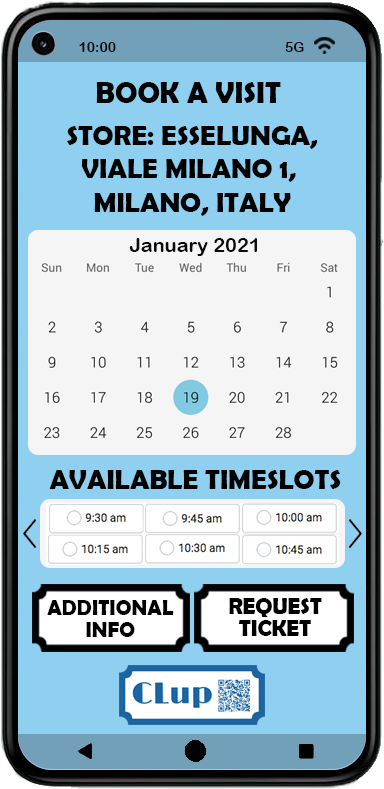
\includegraphics[width=0.65\textwidth]{Images/App/Android_BookAVisit}
\caption{\label{fig:androidbav}\textbf{App "Book a visit" screen}}
\end{figure}
\end{itemize}
\newpage


\begin{itemize}
\item Additional info screen when booking a visit. A user can enter estimated shopping time, and if their location is on, Google Maps will estimate the distance to the store and calculate the total time it takes to get there and do the shopping.
\begin{figure}[!htb]
\centering
\begin{minipage}{0.4\textwidth}
\centering
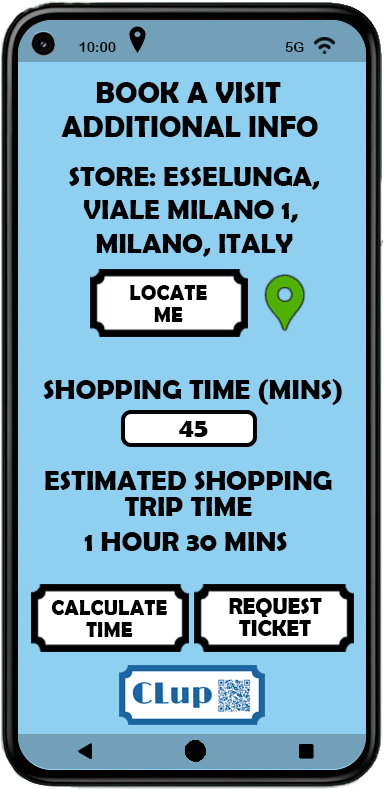
\includegraphics[width=0.65\textwidth]{Images/App/Android_AdditionalInfoYesLoc}
\caption{\label{fig:androidinfoloc}\textbf{App additional info screen (location on)}}
\end{minipage}
\begin{minipage}{0.4\textwidth}
\centering
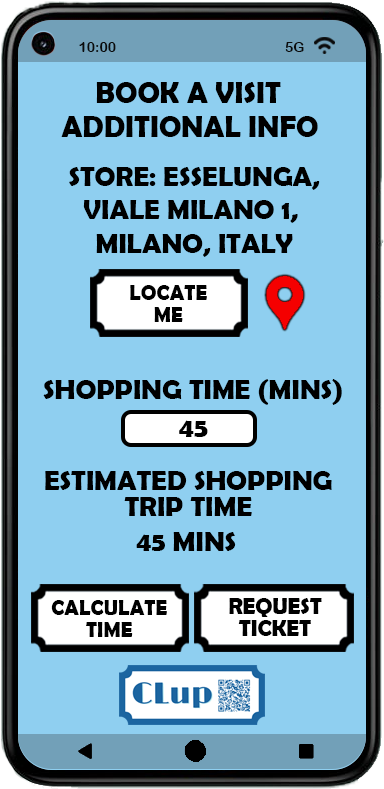
\includegraphics[width=0.65\textwidth]{Images/App/Android_AdditionalInfoNoLoc}
\captionsetup{justification=centering}
\caption{\label{fig:androidinfonoloc}\textbf {App additional info screen (location off)}}
\end{minipage}
\end{figure}

\item Screen featured when a store manager is logged in. Both examples of a valid ticket scan and an invalid ticket scan are shown.
\begin{figure}[!htb]
\centering
\begin{minipage}{0.4\textwidth}
\centering
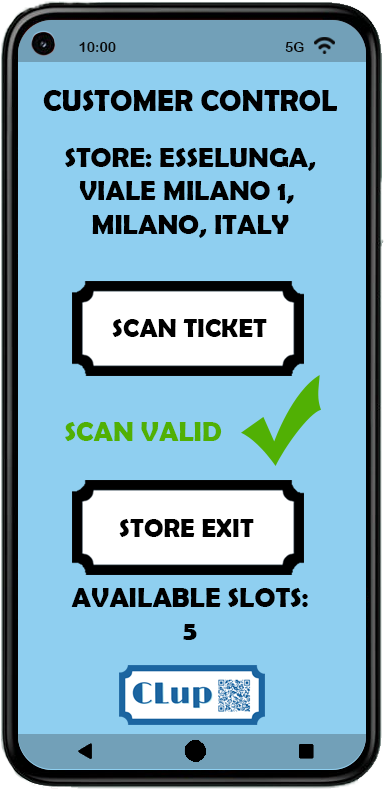
\includegraphics[width=0.65\textwidth]{Images/App/Android_ValidScan}
\caption{\label{fig:androidvalidscan}\textbf{App store manager screen (valid scan)}}
\end{minipage}
\begin{minipage}{0.4\textwidth}
\centering
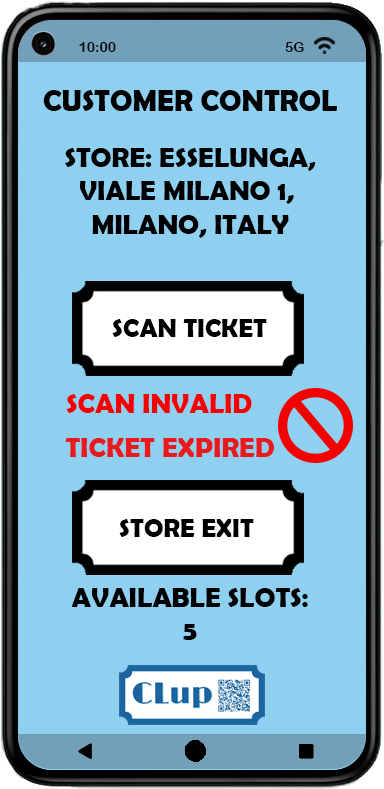
\includegraphics[width=0.65\textwidth]{Images/App/Android_InvalidScan}
\captionsetup{justification=centering}
\caption{\label{fig:androidinvalidscan}\textbf {App store manager screen (invalid scan)}}
\end{minipage}
\end{figure}
\end{itemize}


